\section{Filtro Popart}
\subsection{Enunciado}

\subsection*{Filtro \textit{Popart}}

  Programar el filtro \textit{Popart} en lenguaje C y en en ASM haciendo uso de 
  las instrucciones vectoriales (\textbf{SSE}).

\vspace*{0.3cm} \noindent
\textbf{Experimento 1 - saltos condicionales}

	Se desea conocer que tanto impactan los saltos condicionales
	en el código del ejercicio anterior con \verb|-O1|.\\
	Para poder medir esto, una posibilidad es quitar las comparaciones
	al procesar cada pixel. Por más que la imagen resultante no sea correcta,
	será posible tomar una medida del impacto de los saltos condicionales.
	Analizar como varía la performance. 
	
	Si se le ocurren, mencionar otras posibles formas de medir el impacto de los saltos condicionales.

\vspace*{0.3cm} \noindent
\textbf{Experimento 2 - cpu vs. bus de memoria}

	¿Cuál es el factor que limita la performance en este caso? 
	
	Realizar un experimento, agregando múltiples instrucciones de un mismo tipo
	y realizar un análisis 	del resultado. Acompañar con un gráfico.


\vspace*{0.3cm} \noindent
\textbf{Experimento 3 - prefetch}

  La técnica de \textit{prefetch} es otra forma de optimización que puede
  realizarse. Su sustento teórico es el siguiente:
  
  Suponga un algoritmo que en cada iteración tarda n ciclos en obtener un dato y una cantidad
  similar en procesarlo. Si el algoritmo lee el dato $i$ y luego lo procesa,
  desperdiciará siempre n ciclos esperando entre que el dato llega y que se comienza
  a procesar efectivamente. Un algoritmo más inteligente podría pedir el 
  dato $i+1$ al comienzo del ciclo de proceso del dato $i$ (siempre suponiendo
  que el dato $i$ pidió en la iteración $i-1$. De esta manera, a la vez que el
  procesador computa todas las instrucciones de la iteración $i$, se estáran trayendo
  los datos de la siguiente iteración, y cuando esta última comience, los datos ya
  habrán llegado.

  \vspace*{0.2cm}
  Estudiar esta técnica y proponer una aplicación al código del filtro en la versión ASM.
  Programarla y analizar el resultado. ¿Vale la pena hacer prefetching?

\vspace*{0.3cm} \noindent
\textbf{Experimento 4 - secuencial vs. vectorial}

  Analizar cuales son las diferencias de performace entre las versiones de C y ASM. 
  Realizar gráficos que representen estas diferencias.


\subsection{An\'alisis previo}
El algoritmo de popart reemplaza cada pixel por uno de cinco pixeles preseleccionados. 
La elecci\'on resulta de la suma de los elementos del pixel.

En un primer an\'alisis, el filtro popart tiene 3 partes: el ciclo, la suma de los elementos rgb, y la elecci\'on del pixel de reemplazo.

\subsection{Implementaci\'on en C}
Para la implementaci\'on en C usamos un vector con los posibles reemplazos para cada pixel, 
y una funci\'on que devuelve cual va a ser ese reemplazo mediante comparaciones.
\begin{codesnippet}
\begin{verbatim}

rgb_t colores[] = { {255,   0,   0},
                    {127,   0, 127},
                    {255,   0, 255},
                    {  0,   0, 255},
                    {  0, 255, 255} };

			
int pop_art(unsigned int r, unsigned int g, unsigned int b)
{
    unsigned int suma = r + g + b;
    int res;
	
    if 		 (suma < 153)	{res = 0;}
    else if (suma < 306)	{res = 1;}
    else if (suma < 459)	{res = 2;}
    else if (suma < 612)	{res = 3;}
    else 					{res = 4;}
	
    return res;
}
\end{verbatim}
\end{codesnippet}

\subsection{Implementaci\'on en assembler}
Armamos máscaras para las comparaci\'ones con suma(i,j).
\begin{codesnippet}
\begin{verbatim}
seisDoce:          DD 0x264, 0x264, 0x264, 0x264    ; 612, 612, 612, 612			
cuatroCincoNueve:  DD 0x1CB, 0x1CB, 0x1CB, 0x1CB    ; 459, 459, 459, 459	
tresOSeis:         DD 0x132, 0x132, 0x132, 0x132    ; 306, 306, 306, 306	
unoCincoTres:      DD 0x99, 0x99, 0x99, 0x99        ; 153, 153, 153, 153
\end{verbatim}
\end{codesnippet}

Tambi\'en para reemplazar los pixeles (solo cito el primer caso).
\begin{codesnippet}
\begin{verbatim}
colores0:          DB  0xFF, 0x0,  0x0, 0x0,        ; 255,   0,   0,   0
                   DB  0xFF, 0x0,  0x0, 0x0,        ; 255,   0,   0,   0
                   DB  0xFF, 0x0,  0x0, 0x0,        ; 255,   0,   0,   0
                   DB  0xFF, 0x0,  0x0, 0x0         ; 255,   0,   0,   0

\end{verbatim}
\end{codesnippet}
El resto de las m\'ascaras, usadas con \verb|PSHUFB|.\\ son:

\begin{itemize}
	\item pixel0BGR : Para tener un pixel (R,G y B) en cada \textit{double word}. El cuarto Byte se rellena con ceros
			
	\item soloPrimero : Lo usamos para trabajar sobre el primer Byte de cada \textit{double word}
		
	\item pixelFinal : Sirve para sacar el ceros ubicado en el cuarto Byte de cada \textit{double word}. El ultimo DB se rellena con ceros
\end{itemize}
\'Estas m\'ascaras son usadas en \textit{pop_art} para discriminar los Bytes de R, G y B y guardar la suma de cada uno en un \textit{double word}

El uso de \textit{double word} viene del hecho de que un pixel se compone de tres elementos de un Byte cada uno, 
y necesitamos tener cada pixel en una cantidad par de Bytes para poder desempaquetar correctamente. Esto nos lleva a usar 4 Bytes por cada pixel.

Otra parte del codigo importante es el que genera la sumatoria, para lo cual utilizamos los \verb|PSHUFB|:\\
\begin{codesnippet}
\begin{verbatim}
	MOVDQU XMM0, [RDI]	; R|G|B|R|G|B|R|G|B|R|G|B|R|G|B|R coloco los primeros 16bytes 
                        ; de la imagen en XMM1

    XORPD XMM2, XMM2
    XORPD XMM3, XMM3
    XORPD XMM4, XMM4
    MOVDQA XMM7, [pixel0BGR]
    PSHUFB XMM0, XMM7              ; ordeno en el registro los pixels de forma 0RGB 
                                   ; (tengo 4 pixeles)
    MOVDQU XMM2, XMM0              ; XMM2: R|G|B|0|R|G|B|0|R|G|B|0|R|G|B|0
    PSHUFB XMM2, [soloPrimero]     ; XMM2: R|0|0|0|R|0|0|0|R|0|0|0|R|0|0|0
                                   ; solo dejamos azul para 'suma'
    MOVDQU XMM3, XMM0              ; XMM3: R|G|B|0|R|G|B|0|R|G|B|0|R|G|B|0 	
    PSRLD XMM3, 8                  ; XMM3: G|B|0|0|G|B|0|0|G|B|0|0|G|B|0|0		
    PSHUFB XMM3, [soloPrimero]     ; XMM3: G|0|0|0|G|0|0|0|G|0|0|0|G|0|0|0
                                   ; solo dejamos verde para 'suma'
    MOVDQU XMM4, XMM0              ; XMM4: R|G|B|0|R|G|B|0|R|G|B|0|R|G|B|0 	
    PSRLD XMM4, 16                 ; XMM4: B|0|0|0|B|0|0|0|B|0|0|0|B|0|0|0
                                   ; solo dejamos rojo para 'suma'
    ;Ahora podemos hacer suma
    PADDW XMM2, XMM3
    PADDW XMM2, XMM4               ; XMM2: dword[R+G+B] dword[R+G+B] dword[R+G+B] dword[R+G+B]
\end{verbatim}
\end{codesnippet}

\subsection{Resultado de los experimentos}
%\begin{figure}
%  \begin{center}
%	
\includegraphics[scale=0.66]{imagenes/logouba.jpg}
%	\caption{Logo}
%	\label{Logo}
%  \end{center}
%\end{figure}
\vspace*{0.3cm} \noindent
\textbf{Experimento 1 - saltos condicionales}

\vspace*{0.3cm} \noindent
\textbf{Experimento 2 - cpu vs. bus de memoria}

\vspace*{0.3cm} \noindent
\textbf{Experimento 3 - prefetch}

\vspace*{0.3cm} \noindent
\textbf{Experimento 4 - secuencial vs. vectorial}

\begin{figure}
  \begin{center}
	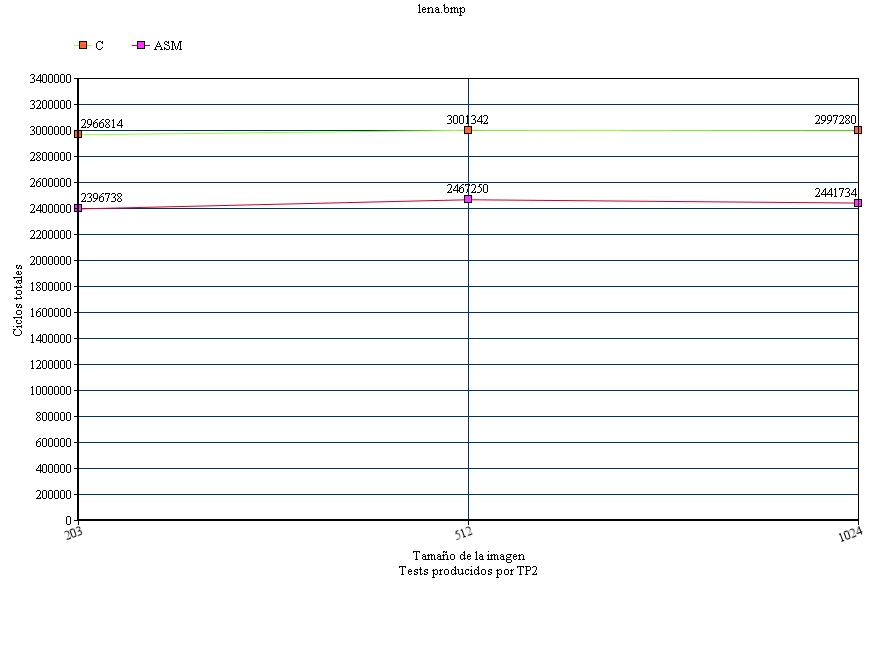
\includegraphics[scale=0.66]{imagenes/ldr-lena.jpg}
	\caption{Lena}
	\label{Lena}
  \end{center}
\end{figure}

\begin{figure}
  \begin{center}
	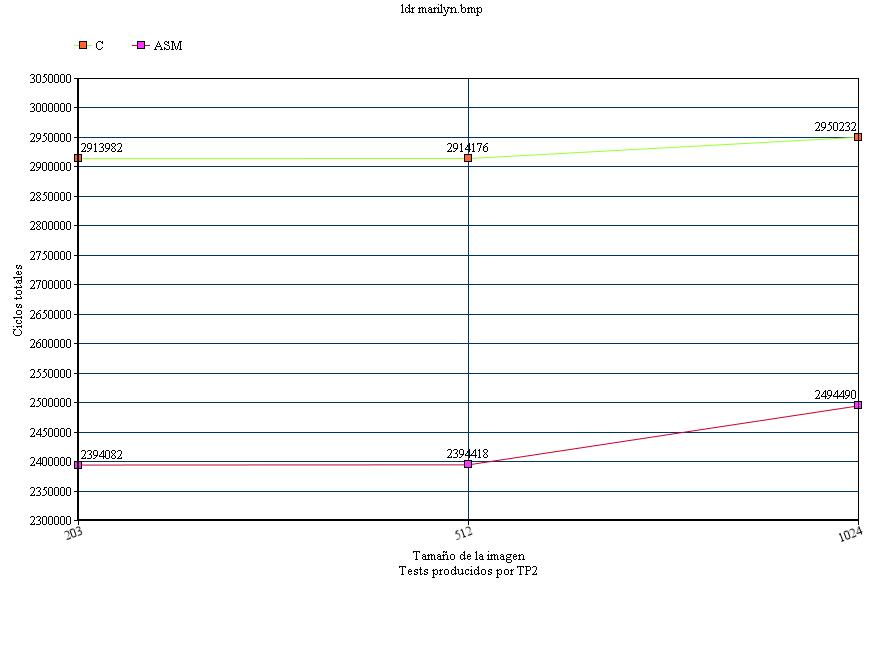
\includegraphics[scale=0.66]{imagenes/ldr-marilyn.jpg}
	\caption{Marilyn}
	\label{Marilyn}
  \end{center}
\end{figure}

Realizamos los tests armando un ciclo de 100000 ejecuciones del mismo c\'odigo con las mismas entradas, y a su vez ejecutamos estos tests 5 veces para cada entrada. \'Esto nos 
permiti\'o hacer promedios y descartar tests que daban muy lejos del valor medio.

Como muestran los gr\'aficos presentados, hay claras diferencias de velocidad (medida en cantidad de ciclos) entre uno y otro lenguaje. Tambi\'en notamos que no hay una gran 
variaci\'on de velocidad entre los distintos tamaños de las im\'agenes, as\'i como a veces las variaciones no son las esperadas. En este sentido, realizamos varias ejecuciones 
del TP2 con exactamente los mismos par\'ametros y vimos que variaban sin un patr\'on. Pensamos que si mejoraba con las sucesivas iteraciones podr\'ia ser 
producto de la acci\'on de la cache, pero como no fue as\'i vemos que tiene que ver con qu\'e tan ocupado est\'a el cpu. \'Esto no pudo ser confirmado ya que todos 
los tests se corrieron sin que ningun otro programa visible a nosotros est\'e corriendo.
\begin{figure}
  \begin{center}
	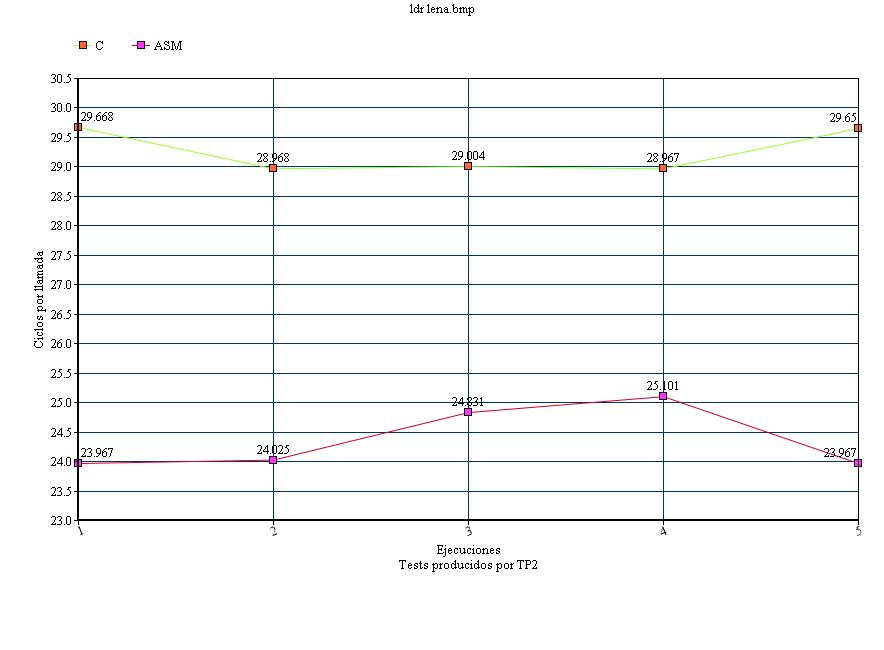
\includegraphics[scale=0.66]{imagenes/ldr-lena-203.jpg}
	\caption{lena-203x203}
	\label{lena-203x203}
  \end{center}
\end{figure}
